%% Estuarine, Coastal and Shelf Science — elsarticle, author-year (Harvard)
%% Review mode: double-spaced, line numbers, single column.
%% Preamble mirrors reservoirs_s1_svm/manuscript/main.tex (Paper 1 and Paper 2).
\documentclass[review,12pt,authoryear]{elsarticle}

%% --- Encoding & fonts ---
\usepackage[T1]{fontenc}
\usepackage[utf8]{inputenc}
\usepackage{lmodern}

%% --- Math ---
\usepackage{amsmath,amssymb}

%% --- Graphics & tables ---
\usepackage{graphicx}
\graphicspath{{figures/}}
\usepackage{float}
\usepackage{booktabs}
\usepackage{tabularx}
\usepackage{longtable}
\usepackage{multirow}

%% --- Hyperlinks ---
\usepackage[hidelinks]{hyperref}
\usepackage{url}

%% --- Units ---
\usepackage{siunitx}
\sisetup{detect-all, group-separator={,}}

%% --- Misc ---
\usepackage{microtype}
\usepackage{lineno}       % line numbers (activated by 'review' class option)
\usepackage{setspace}
\usepackage[margin=2.5cm]{geometry}

%% --- Bibliography (natbib, Harvard author-year) ---
\biboptions{authoryear,round,semicolon}

% -----------------------------------------------------------------------
\begin{document}

\begin{frontmatter}

\title{Transport validation of a wave-coupled lagoon model: interacting
       effects of seagrass roughness and bed mobility}

\author[unipa]{Cicero Martins Jr.\corref{cor1}}
\ead{cicero.martinsjr@unipa.it}

\author[unipa]{Giuseppe Ciraolo}
\author[unipa]{Mauro De Marchis}

\cortext[cor1]{Corresponding author}
\affiliation[unipa]{organization={Dipartimento di Ingegneria,
                    Università degli Studi di Palermo},
                    city={Palermo},
                    country={Italy}}

% -----------------------------------------------------------------------
\begin{abstract}
%% 220 words. ECSS limit is 250 (confirmed 2026-08-07). Not the 150-word ENVSOFT
%% cap that applies to the reservoirs manuscripts.
Coastal lagoon models are routinely validated against water level, yet water
level may constrain transport weakly. We test this in the Stagnone di Marsala,
a micro-tidal Sicilian lagoon of sub-metre mean depth colonised by
\emph{Posidonia oceanica}, using a three-dimensional Delft3D Flexible Mesh model
coupled to SWAN over nine days of July 2025. A complete factorial in wave
coupling, bed mobility and whether seagrass resistance is uniform or distributed
from a satellite classification gives eight configurations, each scored against
three tide gauges and 35 GPS surface drifters. The eight are indistinguishable
in water level, with anomaly RMSE differing by at most four millimetres, while
their Liu--Weisberg skill spans 0.469 to 0.705 and their endpoint separation 336
to 625~m. Neither wave coupling nor bed mobility improves Lagrangian skill on
its own, and each is what makes the other work. Wave coupling on a fixed bed
costs 0.035 to 0.042; bed mobility without waves costs 0.071 to 0.075 and makes
every drifter worse; together they gain 0.119 to 0.232. The two worst and the
two best configurations are built from the same pair of treatments. Distributed
roughness is a third-order refinement that pays only when both are present.
Completing the factorial was necessary rather than tidy: measured on a fixed bed
alone, wave coupling appears to be a consistent small penalty, and the sign
inverts in the cells that a partial design omits.
\end{abstract}

%% ECSS allows 1-7 keywords. Avoid multi-word keywords joined by 'and'/'of'.
\begin{keyword}
Coastal lagoon \sep
Delft3D Flexible Mesh \sep
Morphodynamics \sep
\emph{Posidonia oceanica} \sep
Lagrangian drifters \sep
Three-dimensional circulation
\end{keyword}

\end{frontmatter}

\linenumbers   % activate line numbering for review

% -----------------------------------------------------------------------
\section{Introduction}
\label{sec:introduction}

Coastal lagoons are among the most productive coastal environments on Earth.
Their shallow, semi-enclosed geometry concentrates fisheries and biodiversity
along roughly 13\% of the global shoreline \citep{Carrasco2016, Kjerfve1994},
while making these systems acutely sensitive to the atmospheric and tidal
forcing that drives water exchange and renewal. In the Mediterranean basin,
where tidal amplitudes rarely exceed 0.3~m, the balance among tidal
oscillations, wind stress, and seiche phenomena varies considerably among
systems, yet wind consistently emerges as a significant driver of horizontal
exchange and a key modulator of the residence times and salinity gradients
that condition benthic habitat \citep{Niedda2007, Umgiesser2014}. The presence
of dense submerged vegetation, principally \emph{Posidonia oceanica} (L.)
Delile and \emph{Cymodocea nodosa} (Ucria) Ascherson along Mediterranean
shores, introduces a further layer of complexity. Seagrass canopies attenuate
incident wave energy \citep{Infantes2012} and extract momentum from the mean
flow through canopy drag, modifying near-bed turbulence and the vertical
velocity structure \citep{Nepf2012}. As global seagrass extent continues to
decline at accelerating rates \citep{Waycott2009}, understanding how
circulation controls residence times, dispersal, and habitat connectivity in
vegetated coastal systems has become an urgent scientific and management
priority. Addressing it requires circulation models that accurately reproduce
transport pathways rather than water levels alone, and this distinction makes
Lagrangian validation essential. By tracking the cumulative separation between
simulated and observed drifter trajectories over time, the Lagrangian skill
score provides a direct and discriminating measure of model accuracy that
conventional scalar metrics cannot replicate
\citep{Liu2011, Revelard2021}.

The \emph{Stagnone di Marsala}, on the north-western coast of Sicily, offers a
natural laboratory for these questions. The lagoon extends approximately 11~km
in the north--south direction and 2.5~km east--west, enclosing a surface area
of roughly 2200~ha between the mainland and the elongated Isola Grande
\citep{DeMarchis2012}. Its mean water depth is approximately 0.95~m, ranging
from a few tens of centimetres over the northern intertidal flats to a maximum
of about 3~m near the southern inlet, placing it firmly in the class of very
shallow coastal systems in which the depth-averaging assumption is, a priori,
difficult to justify. Hydrodynamic exchange with the open Mediterranean is
mediated by two mouths of strongly contrasting geometry: a narrow northern
inlet ($\sim$400~m wide, 0.30--0.40~m deep) whose shallow sill severely
restricts tidal exchange, partially mitigated by a historically dredged
channel, and a wide southern inlet ($\sim$2900~m wide, 1.0--1.5~m deep) that
controls the bulk of mass transfer
\citep{DeMarchis2012, CiraoloDeMarchis2009}. The lagoon supports no
significant freshwater input, and its bottom is colonised by
\emph{P.\ oceanica} in the central and southern basin and by
\emph{C.\ nodosa} in the shallower northern reaches, with shoot densities
reaching 1000--1200 plants~\si{\per\metre\squared} \citep{Ciraolo2009a}.
Designated as a \emph{Riserva Naturale Orientata} and a Natura 2000 site, the
Stagnone hosts recognised populations of protected flora and fauna. Despite
this status, satellite monitoring over 2003--2024 has documented a 75\%
reduction in the extent of the \emph{P.\ oceanica} atoll and cordon formations
\citep{Maltese2025}, underscoring the need to understand the hydrodynamic
processes that govern conditions within this enclosed basin.

The tidal regime is microtidal, with free-surface amplitudes of the order of
0.25~m dominated by semi-diurnal harmonics \citep{DiMarca2009}. In the absence
of riverine input and with weak tidal forcing, circulation is driven almost
exclusively by tidal oscillations and wind stress. Field experiments and 3D
numerical modelling conducted by \citet{DeMarchis2012} during a July 2006
campaign showed that tidal action dominates north--south exchange, while wind
is the controlling agent of east--west currents and, critically, generates
pronounced vertical recirculation structures entirely absent in tide-only
simulations. This established that vertical velocity shear between wind-driven
surface drift and near-bed return flow is quantitatively significant even at
sub-metre depths, and that the tendency towards hypersaline conditions in
summer \citep{LaLoggia2004} adds a baroclinic component that reinforces
stratification in the vertical.

Prior numerical investigations of the Stagnone have employed both
depth-averaged and three-dimensional approaches, each appropriate to the
research objective pursued. \citet{LaLoggia2004} and \citet{DiMarca2009}
applied 2D depth-averaged models to characterise tidal flushing, residence
times, and turbidity dynamics, yielding useful insight into the basin-scale
water budget and the role of biological productivity in light attenuation.
\citet{Ciraolo2009a} demonstrated through particle tracking the sensitivity of
simulated trajectories to the assumed velocity field, highlighting the
importance of current accuracy for transport prediction.
\citet{DeMarchis2012} showed that resolving the vertical dimension is
necessary to reproduce wind-driven recirculation. Their 3D non-hydrostatic
finite-volume model, validated against simultaneous velocity and water-level
measurements at multiple stations, achieved substantially better agreement
with observed east--west currents than any depth-averaged simulation. More
recently, \citet{Ingrassia2024} returned to a 2D unstructured-mesh framework
(MIKE 21) and conducted systematic sensitivity tests of bed friction, varying
the Gauckler--Strickler coefficient uniformly across the lagoon for different
vegetation scenarios. The value $K_s = 20$~m$^{1/3}$~s$^{-1}$ was identified
as most representative for the vegetated basin, yielding Nash--Sutcliffe
efficiencies up to 0.92 for water level. The authors noted that the 2D
approximation remains adequate for large-scale water-level budgeting while
acknowledging reduced predictive skill for horizontal velocity, particularly
in the northern, shallower sub-basin.

Building on these foundations, the present study addresses two aspects that
have not yet been incorporated jointly into a Stagnone circulation model. The
first is wave--current coupling. Spectral ocean waves generated in the western
Sicilian channel can penetrate both inlets and interact with the mean flow,
altering near-bed turbulence and the effective drag experienced by the
seagrass canopy. Coupled wave and flow modelling in comparably shallow
Mediterranean basins has shown this to be non-negligible. In the Venice Lagoon
\citet{Carniello2011} found the wave-induced contribution to bed shear stress
to interact non-linearly with the current-induced contribution, so that neither
can be obtained from the other. In the Mar Menor, a restricted micro-tidal
lagoon of comparable depth, \citet{Morote2025} found locally generated waves to
produce near-bed orbital velocities sufficient to mobilise bottom sediment over
most of the basin. Neither process has been represented in previous Stagnone
simulations. The second is the combined use of spatially distributed vegetation
roughness mapped from satellite imagery, rather than assumed uniform, and
Lagrangian drifter observations as a validation target. Together, these extensions allow the relative contributions
of three-dimensional dynamics, wave forcing, and seagrass heterogeneity to
transport skill to be quantified within a controlled process-attribution
framework.

We apply the three-dimensional unstructured-mesh hydrodynamic solver Delft3D
Flexible Mesh (D-Flow FM; \citealp{Kernkamp2011}) coupled online with the
spectral wave model SWAN \citep{Booij1999}, driven by ERA5 reanalysis
meteorological forcing and CMEMS Mediterranean physical reanalysis boundary
conditions, over a nine-day period in July 2025. The seagrass canopy is
represented as a three-dimensional drag field resolved per sigma layer, with
its parameters taken from published flume and large-scale measurements of the
same species and its spatial distribution from a supervised random-forest
classification of PlanetScope multispectral imagery acquired in August 2023,
following the mapping methodology of \citet{Maltese2025}. Model performance is assessed against in-situ water level
time series at three lagoon stations and an offshore tide gauge, and against
GPS surface drifter trajectories from a field campaign concurrent with the
simulation period, using the Liu--Weisberg Lagrangian skill score and endpoint
proximity as metrics. A complete $2\times2\times2$ factorial in wave coupling,
seagrass canopy and morphodynamic bed update attributes differences in
Lagrangian skill to individual physical mechanisms and to their interactions
(Section~\ref{sec:methods_experiments}).

The paper is organised as follows. Section~\ref{sec:study_area} describes the
study area and its hydrodynamic setting. Section~\ref{sec:data_methods}
presents the observational datasets, the modelling framework, and the seagrass
mapping and drifter validation methodology. Section~\ref{sec:results} reports
validation results for water level and Lagrangian trajectories and the
process-attribution experiment. Section~\ref{sec:discussion} discusses the
implications for wind-driven vertical structure and seagrass--flow
interaction. Section~\ref{sec:conclusions} provides conclusions.

\section{Study Area}
\label{sec:study_area}

The \emph{Stagnone di Marsala} is located on the north-western coast of
Sicily, sheltered from the western Sicilian channel by Isola Grande, an
elongated barrier island running parallel to the mainland coast
(Figure~\ref{fig:study_area}). The enclosed basin extends approximately 11~km
in the north--south direction and 2.5~km east--west, enclosing a total surface
area of roughly 2200~ha \citep{DeMarchis2012}. Two geomorphologically distinct
sub-basins are separated by a \emph{Posidonia oceanica} barrier reef
\citep{LaLoggia2004}: the northern sub-basin, with a mean depth of
approximately 1~m and extensive intertidal flats, and the deeper southern
sub-basin, with a mean depth of approximately 2~m and a maximum of about 3~m
near the main inlet. Three islands punctuate the interior, the Phoenician
archaeological site of Mothia in the south-central basin and the smaller
islands of Santa Maria and Scola in the central reaches
\citep{CiraoloDeMarchis2009}. Salt pans (\emph{saline}) occupy both margins of
the lagoon, with extensive historic saltworks on the western barrier island
(Isola Grande) and additional pans along the eastern mainland shore in the
area facing Mothia \citep{Basso2008}. They constitute a distinctive shallow
intertidal habitat within the lagoon system.

Hydrodynamic exchange with the open sea occurs through two morphologically
distinct inlets. The northern inlet (approximately 400~m wide, 0.30--0.40~m
deep) is a highly restricted passage whose tidal prism is severely limited by
its shallow sill. A historically dredged channel (20~m wide, 1~m deep)
partially compensates this restriction \citep{CiraoloDeMarchis2009}. The wide
southern inlet (approximately 2900~m wide, 1.0--1.5~m deep) provides the
primary pathway for mass transport and water mixing between the lagoon and the
open sea \citep{CiraoloDeMarchis2009}. The tidal regime is microtidal, with
free-surface amplitudes of approximately 0.30~m dominated by semi-diurnal
harmonics \citep{LaLoggia2004}. In the absence of riverine input, weak tidal
exchange combined with high summer evaporation drives a pronounced salinity
gradient. Annual lagoon-wide salinity spans 33--46~psu \citep{Basso2008}, with
peak summer values approaching 48~psu in the more confined northern sub-basin,
contrasting with near-marine conditions near the southern inlet
\citep{Mancuso2023}. Wind forcing dominates east--west circulation within the
basin, while tidal exchange controls the north--south component
\citep{CiraoloDeMarchis2009, DeMarchis2012}.

The seagrass mosaic covers the majority of the lagoon floor.
\emph{Posidonia oceanica} occupies the central and southern portions of the
basin, forming both continuous meadows and characteristic atoll patterns
(10--20~m in diameter) that grade into reef formations oriented along the
north--south axis. \emph{Cymodocea nodosa} prevails in the shallower northern
reaches, with \emph{Caulerpa prolifera} replacing \emph{P.\ oceanica} locally
where hydrodynamic and sediment conditions deteriorate
\citep{LaLoggia2004, CiraoloDeMarchis2009}. In Mediterranean meadows of this
type, \emph{P.\ oceanica} areal densities typically range from 500 to
1200 plants~\si{\per\metre\squared} \citep{Ciraolo2009a}. The spatial
distribution of submerged vegetation was mapped from satellite imagery by
\citet{CiraoloMaltese2006}. The roughness parametrisation in this study uses
the updated classification by \citet{Maltese2025} as the base map, applied to
the 2023 epoch (Section~\ref{sec:methods_roughness}). The lagoon is designated
both as a \emph{Riserva Naturale Orientata} and as a Natura 2000 site,
reflecting the conservation importance of these meadows, which have
nevertheless declined by approximately 75\% in extent over the past two
decades \citep{Maltese2025}.

The observational dataset used in this study was collected during July 2025
(Figure~\ref{fig:study_area}). Water level was recorded at three stations,
BocaNord (BN) at the northern inlet, BocaSud (BS) near the southern inlet, and
AltaVilaEst (AE) on the eastern flank of the central basin. Wind speed and
direction and atmospheric pressure were measured at two stations, AE (which
also carries a water-level gauge and a water temperature sensor) and Mulino, a
dedicated meteorological station located near the salt pans in the
central-northern area. Water levels at BN, BS, and AE serve as the primary
validation targets for the hydrodynamic model
(Section~\ref{sec:methods_validation}). Open-sea boundary conditions are
prescribed from CMEMS Mediterranean physical reanalysis products
(Section~\ref{sec:methods_forcing}). Offshore model performance is assessed
against the tidal gauge on Marettimo island (JRC TAD 658), approximately 15~km
to the west, which provides a free-surface reference uninfluenced by lagoonal
dynamics. GPS-tracked surface drifters were released in the lagoon interior
over a sub-period coinciding with the simulation window, and their
trajectories form the basis of the Lagrangian validation
(Section~\ref{sec:methods_validation}).

%% TODO Figure 1 (study area map) not yet produced. Needs: lagoon bathymetry,
%% the two inlets, the three islands, the four in-situ stations (BN, BS, AE,
%% Mulino), Marettimo inset, and the drifter release points. Replace the
%% placeholder box below with \includegraphics once the figure exists.
\begin{figure}[H]
  \centering
  \fbox{\parbox[c][6cm][c]{0.9\textwidth}{\centering\textsf{[Figure~1
  placeholder] Study area map: lagoon bathymetry, northern and southern
  inlets, Mothia/Santa Maria/Scola, in-situ stations BN, BS, AE and Mulino,
  drifter release points, Marettimo inset.}}}
  \caption{The Stagnone di Marsala lagoon on the north-western coast of
  Sicily, showing bathymetry, the two inlets, the interior islands, and the
  July 2025 in-situ station network.}
  \label{fig:study_area}
\end{figure}

\section{Data and Methods}
\label{sec:data_methods}

%% NEXT SECTION TO DRAFT. Material for every subsection below already exists in
%% the repository (README.md "Methodology" and "Model version history", the
%% docs/ notes cited per subsection, and the memory entries). Methods rules
%% from the Elsevier editor deck: past tense throughout, enough detail to
%% reproduce, and no commentary or discussion inside Methods.

\subsection{Hydrodynamic model}
\label{sec:methods_model}

%% D-Flow FM 1.2.184 (Suite 2026.01 HMWQ); unstructured mesh, 21k nodes;
%% 10 sigma layers; k-epsilon turbulence; UNESCO density; WGS84.
%% Bathymetry: EMODnet 2024 + Trapani port patch. bedLevType=3.
%% 8 MPI partitions. Source: README.md, docs/fm_2026_gotchas.md.

\subsection{Wave model and coupling}
\label{sec:methods_waves}

%% SWAN nested grids: outer ~400 m (full FM domain) + inner ~100 m (lagoon);
%% 36 directions; JONSWAP friction + vegetation dissipation.
%% DIMR online coupling, ComInterval = 3600 s, ncFormat = 3.
%% Sources: docs/deltares_hdf5_coupling_report.md, memory
%% hdf5_coupling_resolution, fm_cominterval_required_for_dimr_coupling.

\subsection{Boundary and atmospheric forcing}
\label{sec:methods_forcing}

%% CMEMS Mediterranean physical reanalysis (dataset IDs in memory
%% cmems_phy_dataset_ids); per-node Marettimo-anchored water level offset
%% (docs/marettimo_offset_anchor_2025.md, docs/wl_boundary_offset_justification.md);
%% uxuyadvectionvelocitybnd for offshore stability (memory
%% uxuy_bnd_required_for_offshore_stability); ERA5 wind blended with the AE
%% in-situ station; ERA5 evaporation (memory fm_evaporation_convention).
%% Note for drafting: zos is an anomaly about the NEMO rest state, not a
%% geodetic datum (memory cmems_zos_reference_frame).

\subsection{Seagrass roughness parametrisation}
\label{sec:methods_roughness}

%% Baptist (2007) trachytopes via .arl; CRS must be WGS84 to match the mesh
%% (memory arl_crs_must_match_mesh). Base map: Maltese et al. (2025)
%% classification, 2023 epoch. Automated RF/PlanetScope pipeline
%% (scripts/build_planet_rf_v4.py, memory planet2023_maltese_rf_pipeline).
%% Ingrassia et al. (2024) Ks = 20 as the uniform-roughness reference for the
%% baseline ensemble member (memory ingrassia_2024_vr_calibration).

\subsection{Observational data and validation metrics}
\label{sec:methods_validation}

%% Water level at BN, BS, AE (memory insitu_2025-26_inventory); Marettimo
%% offshore cell selection is non-trivial, use (12.0753, 37.9747) with
%% bl < -0.3 m (memory marettimo_validation_cell).
%% Metrics: report raw and anomaly together, RMSE^2 = bias^2 + RMSE_anom^2.
%% Post-spinup window: drop the first simulated day.
%% Lagrangian: Liu-Weisberg normalised cumulative separation skill score and
%% endpoint proximity, 12 deploys July 2025, OpenDrift on regridded surface
%% currents (memory regrid_opendrift_pipeline).

\section{Results}
\label{sec:results}

\subsection{Water level}
\label{sec:res_wl}

Table~\ref{tab:wl} reports water level skill at the three interior stations for
every ensemble member over the post-spinup window. Raw error is dominated by a
positive bias at BocaNord and AltaVilaEst, between 0.09 and 0.18~m, and is
small at BocaSud, between $-0.004$ and $+0.018$~m. Removing the respective
means leaves an anomaly RMSE of 0.021 to 0.045~m at every station in every
member, with correlations from 0.79 to 0.93 and modelled-to-observed standard
deviation ratios from 1.06 to 1.25.

The spread across configurations is small. Anomaly RMSE varies by 0.005~m or
less between members at any given station, and the ordering of members is not
consistent from one station to another. Variable roughness lowers the
AltaVilaEst bias from 0.117 to 0.091~m relative to its own counterpart and
raises the BocaNord bias from 0.172 to 0.177~m.

\begin{table}[H]
  \centering
  \caption{Water level skill by member and station, 2--10 July 2025.
  $\mathrm{RMSE}^2 = \mathrm{bias}^2 + \mathrm{RMSE}_{\mathrm{anom}}^2$. All
  values in metres except the dimensionless ratios.}
  \label{tab:wl}
  \begin{tabular}{llrrrrr}
    \toprule
    Station & Member & RMSE & Bias & RMSE$_{\mathrm{anom}}$ & $r$ & $\sigma_m/\sigma_o$ \\
    \midrule
    BocaNord & no waves    & 0.150 & $+0.146$ & 0.034 & 0.86 & 1.09 \\
             & waves       & 0.170 & $+0.168$ & 0.030 & 0.88 & 1.09 \\
             & + roughness & 0.172 & $+0.170$ & 0.030 & 0.89 & 1.10 \\
             & + morph.    & 0.175 & $+0.172$ & 0.032 & 0.87 & 1.13 \\
             & full        & 0.180 & $+0.177$ & 0.031 & 0.88 & 1.13 \\
    \midrule
    BocaSud  & no waves    & 0.023 & $-0.004$ & 0.023 & 0.91 & 1.06 \\
             & waves       & 0.028 & $+0.018$ & 0.022 & 0.92 & 1.06 \\
             & + roughness & 0.025 & $+0.012$ & 0.023 & 0.92 & 1.07 \\
             & + morph.    & 0.023 & $+0.009$ & 0.021 & 0.93 & 1.08 \\
             & full        & 0.022 & $+0.003$ & 0.022 & 0.93 & 1.09 \\
    \midrule
    AltaVila & no waves    & 0.116 & $+0.108$ & 0.042 & 0.81 & 1.12 \\
    Est      & waves       & 0.136 & $+0.130$ & 0.039 & 0.82 & 1.14 \\
             & + roughness & 0.130 & $+0.124$ & 0.039 & 0.82 & 1.16 \\
             & + morph.    & 0.124 & $+0.117$ & 0.042 & 0.81 & 1.20 \\
             & full        & 0.102 & $+0.091$ & 0.045 & 0.79 & 1.25 \\
    \bottomrule
  \end{tabular}
\end{table}

\subsection{Lagrangian transport}
\label{sec:res_drifters}

Thirty-five drifters across twelve deployments were scored against each member
over the interval each drifter was in the water, which ranged from 0.5 to
7.2~hours. Table~\ref{tab:lagrangian} summarises the four metrics and
Figure~\ref{fig:lagrangian} shows their distribution.

Mean Liu--Weisberg skill was 0.539 without wave coupling, 0.505 and 0.506 for
the two wave-coupled fixed-bed members, 0.570 with morphodynamics alone and
0.659 with both morphodynamics and distributed roughness. Endpoint separation
followed the same ordering, from 549 to 583~m for the first four members and
343~m for the last. At drifter level the five distributions overlap heavily
(Figure~\ref{fig:lagrangian}a), so the ordering of the means rests on paired
comparison rather than on separation between groups.

\begin{table}[H]
  \centering
  \caption{Lagrangian metrics by ensemble member, 35 drifters over twelve
  deployments. Path ratio is simulated over observed path length and speed
  ratio is mean speed along the simulated track over the observed
  0.143~\si{\metre\per\second}, both scored on the interval each drifter was in
  the water.}
  \label{tab:lagrangian}
  \begin{tabular}{lrrrr}
    \toprule
    Member & LW skill & Endpoint sep.\ (m) & Path ratio & Speed ratio \\
    \midrule
    No waves            & 0.539 & 549 & 0.78 & 0.82 \\
    Waves               & 0.505 & 569 & 0.80 & 0.84 \\
    Waves + roughness   & 0.506 & 583 & 0.81 & 0.85 \\
    Waves + morph.      & 0.570 & 566 & 0.75 & 0.76 \\
    Full                & \textbf{0.659} & \textbf{343} & \textbf{0.96} & \textbf{0.99} \\
    \bottomrule
  \end{tabular}
\end{table}

The wave penalty is not carried by a few deployments
(Figure~\ref{fig:lagrangian}b). Skill falls with wave coupling in 28 of the 35
drifters (sign test $p = 0.0005$) and in 10 of the 12 deployments (sign test
$p = 0.039$, Wilcoxon on deployment means $p = 0.043$). The two deployments in
which waves help are internally consistent, with all three of their drifters
improving in each, so they represent a genuine difference in behaviour rather
than scatter. The largest single degradation is $-0.133$ and the largest single
improvement $+0.069$.

The observed drifters travelled at a mean speed of 0.143~\si{\metre\per\second}.
Along their own simulated trajectories the members reached 0.118, 0.121, 0.122,
0.109 and 0.142~\si{\metre\per\second} respectively
(Figure~\ref{fig:lagrangian}c), so only the member combining morphodynamics and
distributed roughness reproduces the observed transport rate. The remainder
fall 15 to 24\% short. The same ordering appears in the fraction of drifters
whose path ratio falls below 0.7, which is 31 to 34\% for the first four
members against 11\% for the fifth.

\begin{figure}[H]
  \centering
  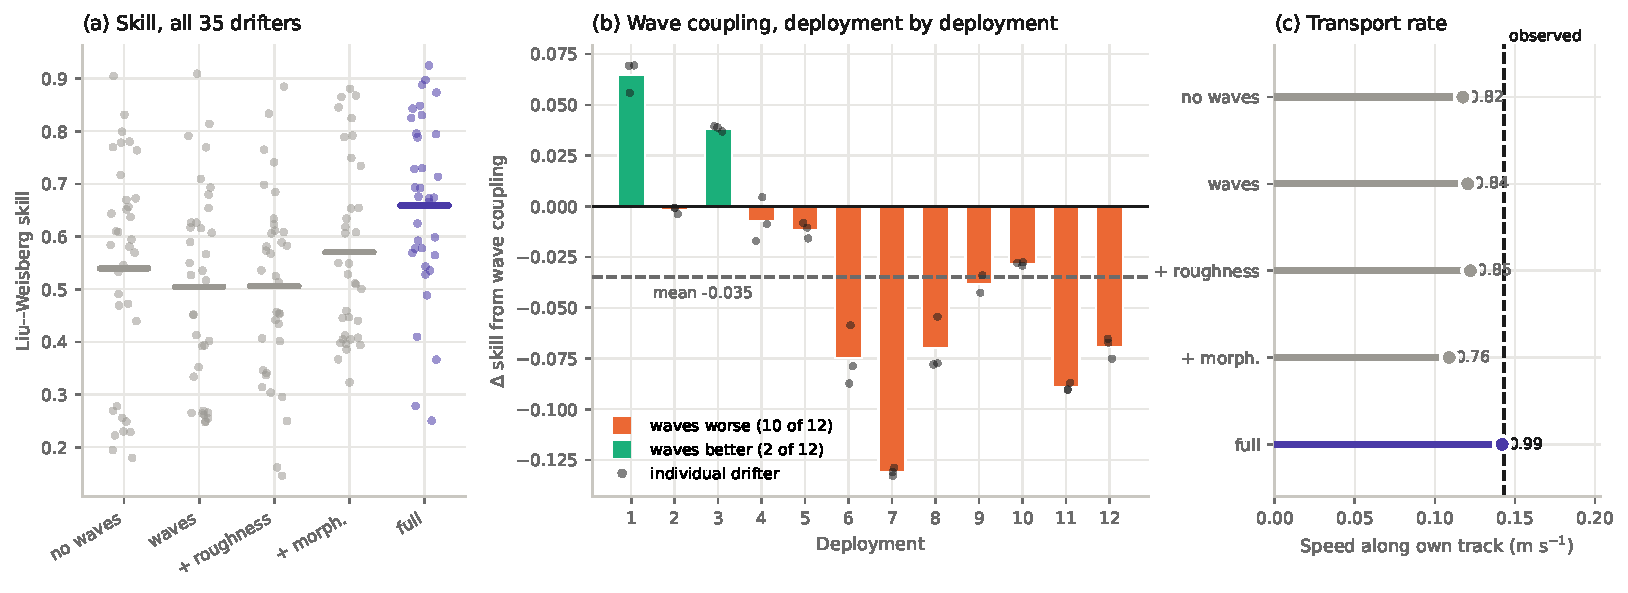
\includegraphics[width=\textwidth]{lagrangian_results}
  \caption{Lagrangian validation. (a) Liu--Weisberg skill for every drifter
  under every member, with the horizontal bar giving the mean. (b) The change
  in skill from wave coupling, by deployment, with individual drifters
  overlaid and the ensemble mean dashed. (c) Mean speed along each member's own
  track against the observed value, with the ratio annotated. The member
  combining distributed roughness and an active bed is drawn in colour
  throughout.}
  \label{fig:lagrangian}
\end{figure}

\subsection{Process attribution}
\label{sec:res_attribution}

Figure~\ref{fig:attribution} gives the paired per-drifter contrasts with
bootstrap confidence intervals. Wave coupling reduces Liu--Weisberg skill by
0.035 (95\% CI $-0.053$ to $-0.017$, $p = 0.001$). Distributed roughness on a
fixed bed changes it by 0.001 (CI $-0.016$ to $+0.018$, $p = 0.34$).
Morphodynamics under uniform roughness changes it by 0.065 (CI $-0.019$ to
$+0.150$, $p = 0.23$). The two contrasts in which both treatments are present
are the only large ones with intervals clear of zero. Distributed roughness
with morphodynamics active gives $+0.089$ (CI $+0.046$ to $+0.133$,
$p < 0.001$), and morphodynamics with distributed roughness active gives
$+0.153$ (CI $+0.056$ to $+0.246$, $p = 0.005$).

Neither treatment produces a demonstrable change on its own and their joint
effect exceeds the sum of the individual point estimates, so the two interact
rather than contribute additively.

The joint effect is not evenly distributed across the dataset. It exceeds
$+0.27$ in five deployments, is close to zero in four, and is negative in
three, reaching $-0.39$ in the deployment with the shortest observed track.

\begin{figure}[H]
  \centering
  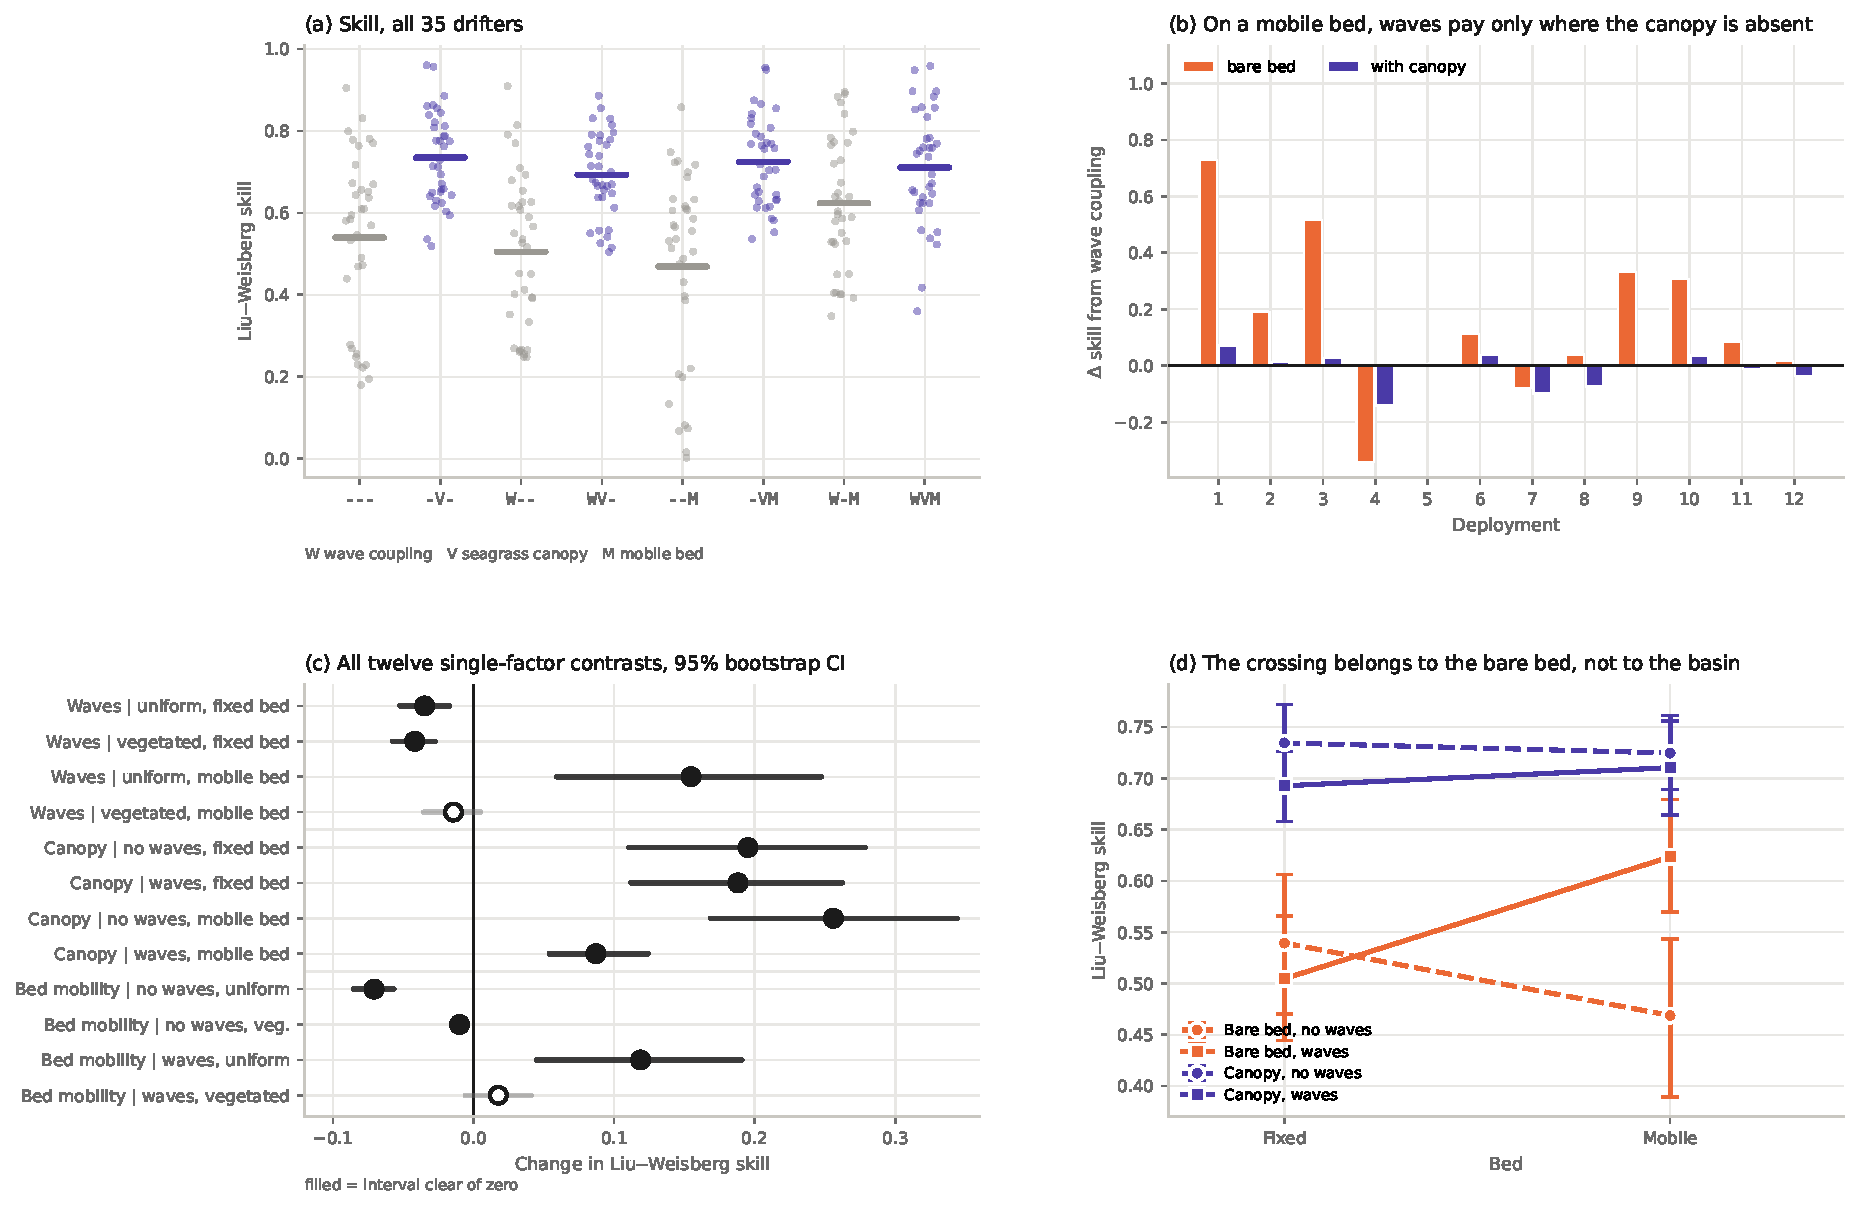
\includegraphics[width=\textwidth]{ensemble_attribution}
  \caption{Process attribution over the ensemble. (a) and (b) give mean skill
  and endpoint separation against the roughness treatment, one line per bed
  treatment, with the no-wave member as the dashed reference and its bootstrap
  interval shaded. (c) gives paired effect sizes with 95\% bootstrap intervals, where
  filled markers denote intervals clear of zero. (d) gives the per-deployment
  mean of the two headline contrasts.}
  \label{fig:attribution}
\end{figure}

\subsection{Three-dimensional structure}
\label{sec:res_3d}

Over 4043 wet cells in the lagoon interior, with the inlets excluded, mean
current speed increases monotonically from the bed to the surface in every
member (Figure~\ref{fig:profile}). Bed-layer speed ranges from 0.021 to
0.040~\si{\metre\per\second} and surface-layer speed from 0.075 to
0.102~\si{\metre\per\second}, giving surface-to-bed ratios of 1.85, 2.07, 2.05,
4.48 and 3.77 across the five members.

The three fixed-bed members give nearly identical profiles, with ratios between
2.05 and 2.07. Both morphodynamic members roughly double the ratio, and they do
so through the bed layer rather than the surface, with near-bed speed falling
from 0.038 to 0.021~\si{\metre\per\second} while surface speed changes by less.
Adding distributed roughness to an active bed lowers surface speed from 0.102
to 0.078~\si{\metre\per\second}.

Lagoon-mean surface speed does not order the members the way transport does.
The member reproducing the observed drifter speed has a lagoon-mean surface
speed of 0.078~\si{\metre\per\second}, below the 0.080 of a member whose
particles travel 15\% too slowly, and below the 0.102 of the member with the
lowest path ratio of all.

\begin{figure}[H]
  \centering
  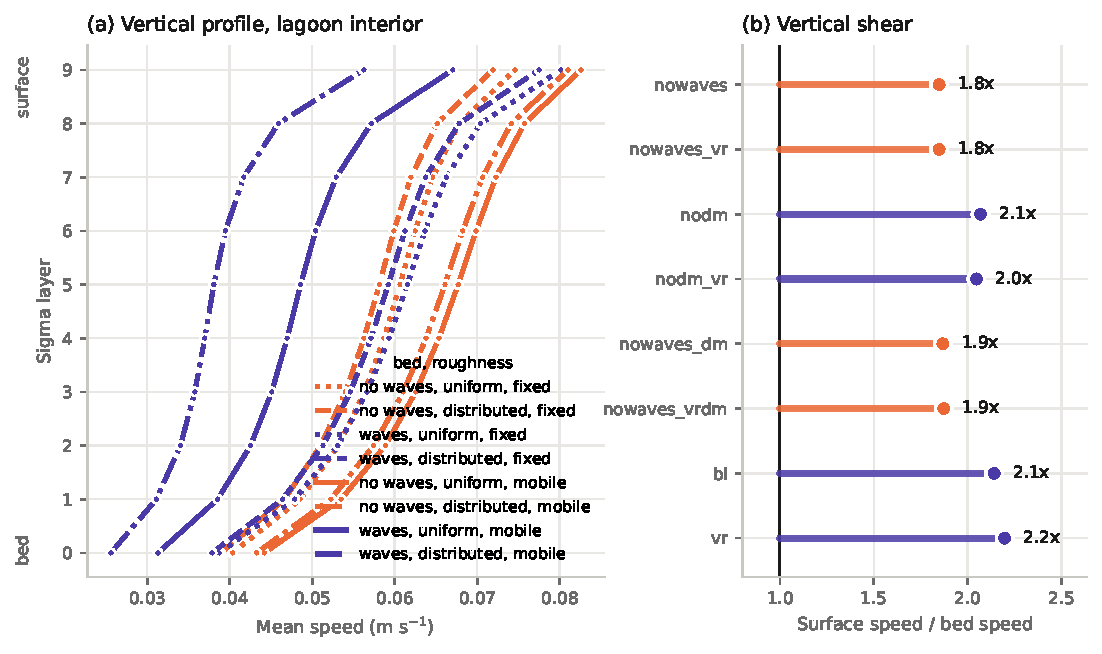
\includegraphics[width=0.88\textwidth]{layer_profile_lagoon}
  \caption{Vertical structure in the lagoon interior over the drifter window.
  (a) Mean speed by sigma layer, colour giving the bed treatment and line style
  the roughness treatment. (b) The ratio of surface to bed speed.}
  \label{fig:profile}
\end{figure}

\subsection{Response of the roughness classes}
\label{sec:res_classes}

Cells were grouped by the trachytope class the model assigned them, taking the
dominant class at the nearest roughness link. Comparing classes within a single
member does not isolate the roughness treatment, because the classes occupy
different parts of the basin at different depths. The uniform-roughness members
make this explicit. With no roughness distinction applied at all, their
\emph{Posidonia} cells are still slower at the bed than their sand cells, in a
ratio of 0.86 and 0.87. The roughness effect is therefore read between members
within a class rather than between classes within a member.

On a fixed bed, moving from uniform to distributed roughness reduces mean bed
speed by 1.3\% over sand, 1.1\% over \emph{Cymodocea}, 3.6\% over
\emph{Posidonia} and 4.5\% over rock (Figure~\ref{fig:classes}b). The effect on
the wave field is larger and ordered as canopy attenuation predicts. Mean
orbital velocity at the bed falls by 11.3\% over sand, 13.7\% over
\emph{Cymodocea} and 14.3\% over \emph{Posidonia}, and by only 3.3\% over rock
(Figure~\ref{fig:classes}c), the rock class being the exposed substrate near
the inlets where mean orbital velocity reaches 0.27~\si{\metre\per\second}
against 0.05 to 0.09~\si{\metre\per\second} elsewhere in the basin.

Introducing bed mobility inverts the class ordering of near-bed speed. The
\emph{Posidonia} to sand ratio rises from 0.85 on a fixed bed to 1.10 and 1.27
in the two morphodynamic members, because sand cells lose roughly half their
near-bed speed while \emph{Posidonia} cells lose about a third.

\begin{figure}[H]
  \centering
  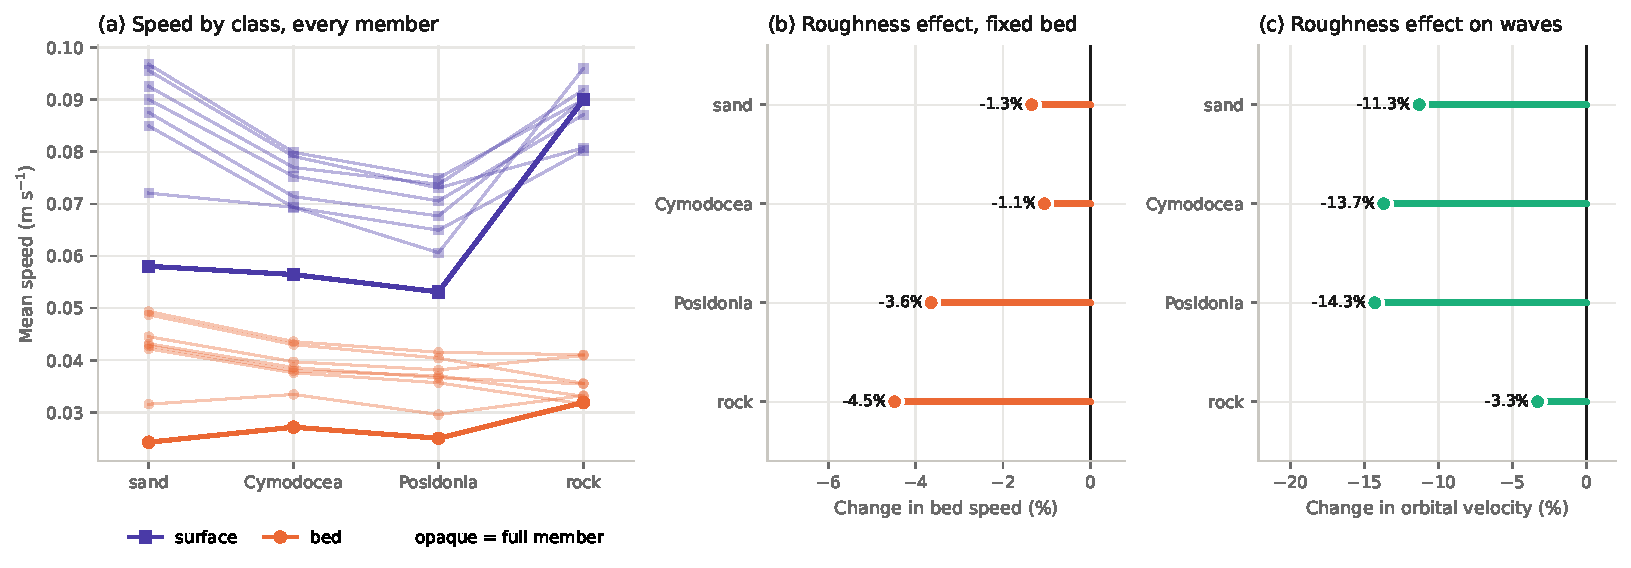
\includegraphics[width=\textwidth]{class_speed_uorb}
  \caption{Flow and wave response by trachytope class in the lagoon interior.
  (a) Mean bed and surface speed by class for every member, the full member
  drawn opaque. (b) Change in mean bed speed from uniform to distributed
  roughness on a fixed bed. (c) The same for mean wave orbital velocity at the
  bed.}
  \label{fig:classes}
\end{figure}

\section{Discussion}
\label{sec:discussion}

\subsection{Water level cannot separate these configurations}

The six members differ in wave coupling, bed mobility and the spatial
treatment of vegetation resistance, and they produce water level records that
are almost the same. Anomaly RMSE varies by six millimetres or less between
members at any station, and no member is consistently best across the three
stations. Over the same simulations Liu--Weisberg skill spans 0.505 to 0.655
and endpoint separation spans 334 to 661~m.

A calibration exercise conducted on water level alone would therefore have no
basis on which to prefer any of these configurations, and would plausibly
select whichever member happened to minimise a station-averaged RMSE by a
margin smaller than the measurement uncertainty. This is the case for treating
Lagrangian observations as a distinct constraint rather than as a confirmation
of a model already tuned to tide gauges. It also suggests that the frequent
practice of reporting coastal model skill through water level statistics alone
may certify transport behaviour that was never examined.

The reason is structural rather than incidental. Water level in a micro-tidal
basin with two open connections is set largely by the offshore forcing and the
basin's capacity to fill and drain, both of which the six members share.
Transport depends on the velocity field, which they do not.

\subsection{Wave coupling}

Wave coupling reduces Lagrangian skill by 0.035 to 0.042, a small effect but a
consistent one, negative in ten of the twelve deployments. It was included in
this model because spectral waves generated in the western Sicilian channel
reach both inlets, and because canopy attenuation is a documented process in
Mediterranean seagrass systems. The result does not contradict either premise.
It says that in this basin, over this window, representing waves did not
improve the prediction of surface transport, and slightly degraded it.

The penalty does not depend on how vegetation resistance is represented. Measured
separately on the two roughness axes it is 0.035 and 0.042, statistically
indistinguishable, with the same consistency across deployments and the same two
deployments improving in both. A single-axis measurement could not have
established that.

One limit remains. The window contains one moderate swell event rather than a
storm, so the test is of ordinary summer conditions, not of the conditions under
which wave effects on transport would be expected to be largest. The wave
contribution is also measured on a fixed bed only, because the mobile-bed
no-wave configurations could not be run, for reasons taken up below.

\subsection{What the interaction acts on}

Neither bed mobility nor distributed vegetation roughness changes Lagrangian
skill by more than a marginal amount on its own: 0.019 for bed mobility under
uniform roughness, 0.001 for roughness on a fixed bed with waves, 0.009 without
them. Applied together they give 0.131 and 0.149 depending on which is held
fixed, improving 32 of the 35 drifters in the first case, and produce the only
configuration that reproduces the observed transport rate, at 0.97 of the
observed path length against 0.78 to 0.93 for the others. The joint effect
exceeds the sum of the separate point estimates by an order of magnitude, which
is the signature of an interaction.

Three candidate explanations for it were tested and rejected before a fourth
line of evidence narrowed the question.

The first was that the roughness field organises where the bed erodes,
producing a channelised bathymetry that conveys flow more efficiently. The
bed-change fields do not support it. Their magnitudes are nearly identical
between the two mobile-bed members, median $-0.059$ against $-0.047$~m in the
lagoon, and their spatial difference is close to zero across the interior. The share of
total bed change held by the busiest 5\% of lagoon cells is 18.9\% and 19.0\%,
indistinguishable, so neither is more focused than the other.

The second was that canopy drag suppresses erosion beneath the meadows. Both
mobile-bed members show more bed change under the canopy than on bare
substrate, in a ratio of 1.49 under uniform roughness and 1.57 under
distributed roughness, so the effect runs in the wrong direction and the
roughness treatment makes it slightly stronger rather than weaker.

The third was that the successful member simply carries a stronger current
field. It does not. Its lagoon-mean surface speed is 0.078~\si{\metre\per\second},
below that of a member whose particles travel 20\% too slowly. The vertical profiles show that
bed mobility, not roughness, controls the shear, and that adding canopy drag to
a mobile bed lowers surface speed rather than raising it.

The particles nevertheless travel at the right speed. Since it is not the mean
speed of the field, it has to be where and when the particles encounter the
faster water, which is a property of the joint space and time structure of the
flow rather than of its magnitude.

Stating this openly is preferable to the available alternative, which is to
attribute the improvement to canopy physics because the successful member is
the one with a canopy. None of the three diagnostics supports that.

The canopy parametrisation does behave as intended, which makes the negative
result sharper rather than weaker. Holding the bed fixed and moving from
uniform to distributed roughness attenuates the wave field in proportion to the
vegetation present, reducing mean orbital velocity at the bed by 14.3\% over
\emph{Posidonia}, 13.7\% over \emph{Cymodocea}, 11.3\% over sand and 3.3\% over
the exposed rock substrate near the inlets. The ordering follows the canopy
density, and the same treatment slows the near-bed flow over \emph{Posidonia}
roughly three times as much as over sand. The vegetation is therefore doing to
the waves and to the bed layer what a canopy should. What it does not do, on a
fixed bed, is change surface transport, and that is the gap the interaction
occupies.

Splitting the trajectory error into a magnitude part and a direction part
narrows where the interaction acts (Figure~\ref{fig:decomp}). For each drifter
the simulated path length, the simulated net displacement and the mean angular
difference between simulated and observed step directions were computed over
the scored window.

The four fixed-bed members are indistinguishable in all three. Path length runs
0.77 to 0.80 of observed, net displacement 0.78 to 0.82, and mean heading error
15.8 to 16.2$^\circ$. Distributed roughness on a fixed bed leaves the heading
error at 16.0$^\circ$, unchanged to the first decimal, so it does not alter
where the particles go any more than it alters how far.

Bed mobility acts mainly on magnitude, raising path length to 0.94 and net
displacement to 0.95, with a smaller gain in heading, to 12.5$^\circ$. Adding
distributed roughness to a mobile bed acts mainly on direction, cutting the
heading error to 8.4$^\circ$, a third of what remained, for a further 0.04 in
path length. The roughness treatment therefore has a directional effect that
exists only when the bed can move, and that is the interaction stated in terms
of what it corrects. Figure~\ref{fig:tracks} shows the same distinction on
individual tracks.

This is a narrowing, not a full account. Treating each track as a single vector
and reconstructing the endpoint separation from the mean displacement ratio and
the mean heading error reproduces the four fixed-bed members within 12\%, at
507 to 538~m against 549 to 583~m observed, but underpredicts the two
mobile-bed members by a factor of 1.4 to 1.9, at 354 and 239~m against 661 and
334~m. A single mean heading is therefore an incomplete description of the
mobile-bed error, and what remains unexplained is why.

\begin{figure}[H]
  \centering
  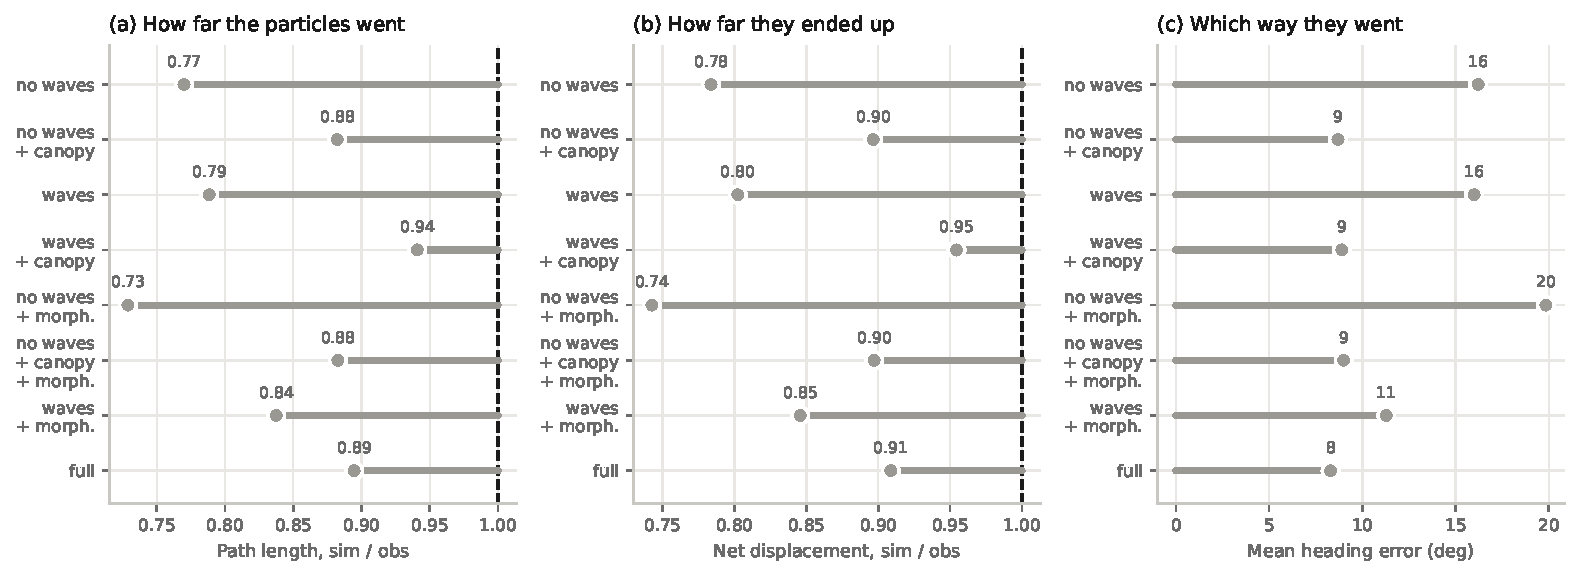
\includegraphics[width=\textwidth]{transport_error_decomposition}
  \caption{The trajectory error split into magnitude and direction. (a) Path
  length and (b) net displacement, both as the ratio of simulated to observed.
  (c) Mean angular difference between simulated and observed step directions.
  The four fixed-bed members coincide in all three panels.}
  \label{fig:decomp}
\end{figure}

\subsection{A mobile bed does not stabilise without waves}

The two ensemble cells combining a mobile bed with no wave coupling could not be
obtained. Both abort on the velocity cap, reaching 27 and
43~\si{\metre\per\second} against a limit of 25, in a single offshore cell and
after roughly half a day of simulation. The four wave-coupled members, carrying
the same sediment settings and the same cap in the earlier configuration, never
approached it.

The behaviour survived the obvious explanation. Morphodynamics initially ran
over the entire domain, including water hundreds of metres deep, and the first
aborts occurred in a cell 27~m deep, so confining sediment to depths above 20~m
was the natural fix. It did not work. With the restriction in place both members
aborted again, at the same cell, at comparable velocities. Restricting the bed
did allow the two wave-coupled mobile-bed members to complete, so the
restriction is not itself the problem.

What this says is that wave coupling performs stabilising work in a
morphodynamic simulation of this basin, and that removing it exposes a feedback
the wave field was otherwise damping. A plausible route is through bed shear
stress, to which waves contribute directly and which sets the erosion rate, so
that removing the wave contribution alters the balance between erosion and the
flow field that drives it. This work does not establish that mechanism, and the
result is reported as an observed property of the configuration.

It also bounds the ensemble. Wave coupling and bed mobility cannot be varied
independently here, so what the design supports is a statement about wave
coupling on a fixed bed and about the roughness-by-bed-mobility interaction
under wave coupling, not a full three-way attribution.

\subsection{The bed-mobility caveat}

The configuration that reproduces observed transport depends on morphodynamics
whose critical shear stress for erosion has not been constrained by a repeated
bathymetric survey. Over nine days the lagoon bed changes by up to 1.0~m in
isolated cells, against a median of 0.05~m, in a basin whose mean depth is
0.95~m. A metre of bed change in nine days is not a physically plausible rate
for this system. The morphodynamic component therefore functions in this
ensemble as a perturbation to the bed whose realism is unverified, and the
interaction reported above should be read with that in mind.

Two readings remain open. Bed mobility may be standing in for a deficiency in
the initial bathymetry, in which case the improvement is a compensation and
would not survive a corrected bed. Or the model may genuinely require an
evolving bed to reproduce transport in a system where the seagrass canopy and
the sediment surface adjust to one another, in which case the calibration
problem is real but the physics is too. Distinguishing them requires
observational constraint on the bed, and satellite-derived bathymetry over
repeated epochs is the most tractable route currently available.

\subsection{Vertical structure}

Surface speed exceeds bed speed by a factor between 1.9 and 4.5 in the lagoon
interior, in a basin whose mean depth is below one metre. Even the weakest case
places a factor of nearly two between the layer a surface drifter samples and
the layer that governs bed shear stress. A depth-averaged representation of
this basin would assign a single velocity to both.

This is consistent with what \citet{DeMarchis2012} found from field
measurements and three-dimensional modelling in the same lagoon, and it
supplies a quantitative basis for the choice of a three-dimensional solver
here. The dependence of the shear ratio on bed mobility, from near 2.0 with a
fixed bed to near 4.0 with a mobile one, also indicates that the vertical
structure is not an independent property of the basin but responds to the same
model choices that govern transport.


\section{Conclusions}
\label{sec:conclusions}

%% Editor-deck rules: not a summary of the paper and no vague future-work
%% outlook. Give global plus specific take-home conclusions, stay quantitative,
%% avoid unnecessary adjectives, and do not duplicate the abstract.


% -----------------------------------------------------------------------
\section*{CRediT authorship contribution statement}
\textbf{Martins Jr, C.:} Conceptualization, Methodology, Software, Formal
analysis, Investigation, Data curation, Visualization, Writing -- original
draft. \textbf{Ciraolo, G.:} Conceptualization, Supervision, Methodology,
Writing -- review \& editing. \textbf{De Marchis, M.:} Conceptualization,
Supervision, Methodology, Writing -- review \& editing.

\section*{Declaration of competing interest}
The authors declare that they have no known competing financial interests or
personal relationships that could have appeared to influence the work reported
in this paper.

\section*{Funding}
%% TODO insert the WETWISE project ID. The application form annex leaves it to
%% the Joint Secretariat, so it is not in the document at
%% Documents/PeriodoAllEstero. UNIPA is partner PP3.
This work was carried out within the project WETWISE, WETland ecosystem
restoration through WISE strategic adaptation across borders, funded by the
Interreg VI-A Italia--Malta Programme under Public Notice 01/2023 and
co-funded by the European Union.

\section*{Acknowledgements}

The authors acknowledge the Copernicus Marine Environment Monitoring Service
(CMEMS) for the Mediterranean physical reanalysis products, the ECMWF for ERA5
atmospheric reanalysis, Planet Labs PBC for the PlanetScope imagery used in
the seagrass classification, and Deltares for the Delft3D Flexible Mesh suite.

\section*{Software and data availability}
\begin{itemize}
  \item \textbf{Model:} Delft3D Flexible Mesh Suite 2026.01 HMWQ (D-Flow FM
  kernel 1.2.184) coupled online with SWAN through DIMR.
  \item \textbf{Source code repository:} \url{https://github.com/cicero-martins/StagnoneDT}
  \item \textbf{Data availability:} ERA5 and CMEMS products are openly
  available from the Copernicus programme. PlanetScope imagery is under
  commercial licence, and scene identifiers are listed in the repository for
  traceability. In-situ water level, wind, and drifter records are archived
  in the repository.
\end{itemize}

%% Generative-AI declaration: withheld by the corresponding author's decision of
%% 2026-08-07, on the grounds that it is not visible in recent ECSS articles.
%% Note that the guide requires it when AI tools were used, and does not condition
%% it on other authors having declared. Restore the block below to include it.
%
% \section*{Declaration of generative AI and AI-assisted technologies in the
% manuscript preparation process}
% During the preparation of this work the authors used Claude (Anthropic) in
% order to assist with drafting and editing the text, with the analysis code used
% to compute the reported diagnostics, and with the preparation of figures from
% model output. After using this tool the authors reviewed and edited the content
% as needed and take full responsibility for the content of the published
% article.

\bibliographystyle{elsarticle-harv}
\bibliography{references}

\end{document}
